% vim: set tw=78 sts=2 sw=2 ts=8 aw et ai:
Having provided an overview on how our solution is designed and how it should
behave, we will now describe the implementation details and obstacles we have
come across. We have implemented a client and a server which hide application
level data in the TCP options field and use it as a command-line interface to
a remote system. We have decided to implement this for Linux systems due to
the fact the Linux system programming interface is extremely flexible and easy
to comprehend.

\subsection{Input and Output}

\subsection{Information Encoding}

Another module of our project is represented by the Encoding module. As we
have previously mentioned, the TCP header options field offers us 37 useful
bytes. Although this is a greater capacity than other protocols offer, it is
still a limited amount, so we have to use it properly.

The first thing to do is minimize the size of the input data (the useful
data encapsulated inside the TCP header), which leads to the idea of compressing
it. Our communication must be reliable and entirely exact, pointing to an
approach based on a lossless data compression algorithm. One of the most
suitable lossless algorithms is Huffman coding.

Huffman coding\cite{huffman1952method} is an entropy encoding algorithm using
a variable-length code table for encoding source symbols (characters in the
current situation), where the table is generated based on the probabilities of
occurence for each of the source symbols. In the end, what you get is a binary
tree of nodes which provides you unique combinations of bits for all the
symbols.

Practically speaking, the compression technique works in the following way:
first, all the nodes are leaf nodes, which contain the symbol itself and the
frequency of occurence; then the nodes are taken two by two starting with the
smallest frequencies, joining them by a common parent containing the sum of
their frequencies; the process is repeated until you have a single root node;
the edges are given bit values (0 the left branches, 1 the right branches);
the encoding for each letter is calculated by following the path of bits from
the root to the corresponding leaf.

\begin{figure}
  \centering
  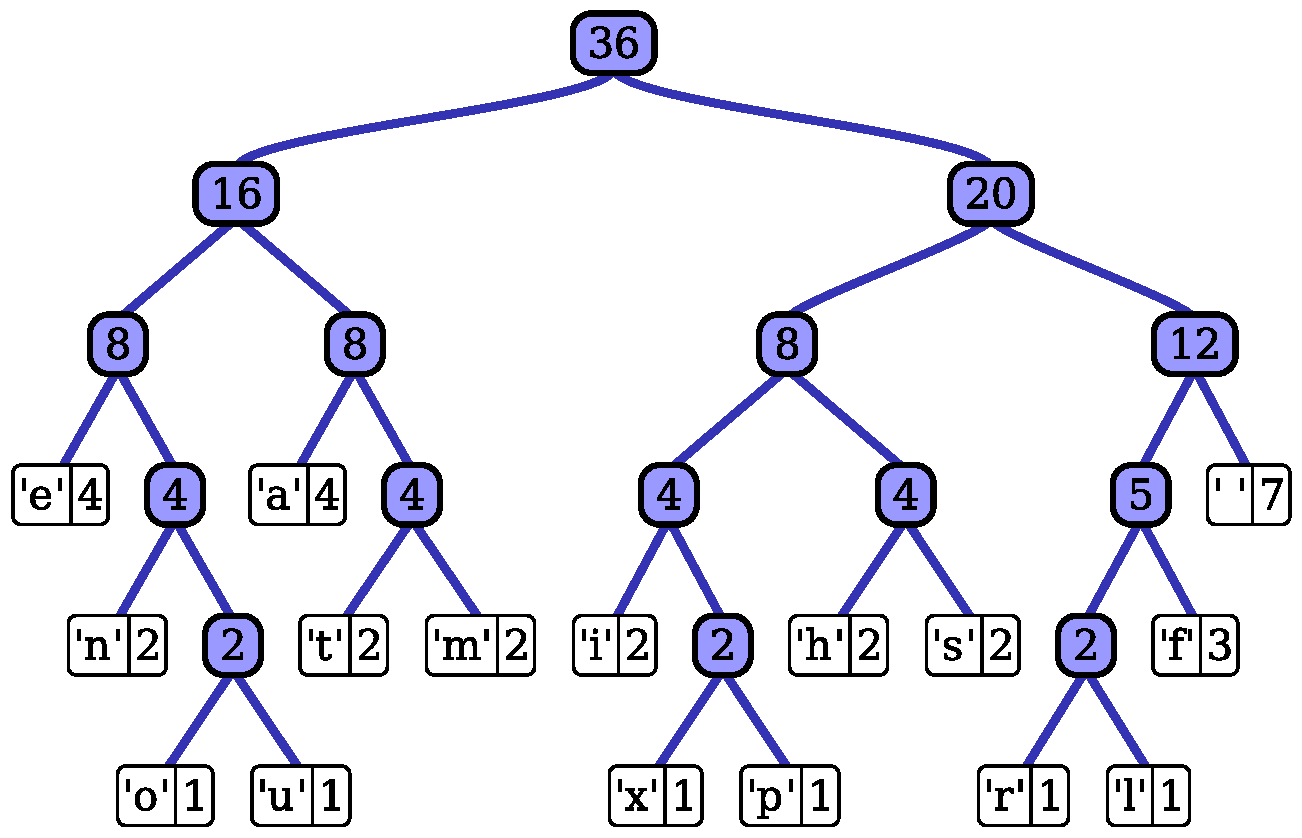
\includegraphics[width=0.5\textwidth]{img/huffman}
  \caption{Huffman tree generated for "this is an example of a huffman tree"}
  \label{fig:huffman}
\end{figure}

Reffering to the example in Figure \ref{fig:huffman}, the code for 'e' would
be '000', for 'a' '010', for 'u' '00111', and so on. As you can see, the most
frequent characters have the shortest codes.

In order to create a working encoding module, we have implemented the Huffman
algorithm to encode / compress the payload of our message. The result is a
sequence of bits to be added in the 37 bytes left of the options field.

But the things weren't that simple. First of all, the message had to be decoded
when it arrived at the destination. For this to be accomplished, we needed to
send the codebook along with the encoded message, so the first bytes of the
field had to define the length of the codebook and describe the codebook itself.

Another problem to overcome was to be continued...

\subsection{Network Communication}

After the Codec module splits the query or response and applies compression,
data is passed to the Net module, which is responsible for encapsulating it in
the TCP header and sending it to the other endpoint.

\begin{lstlisting}[caption={Default TCP Header Structure},
                   label={lst:def-tcphdr},
                   basicstyle=\footnotesize,
                   captionpos=b,
                   frame=single,
                   language=C
                  ]
typedef struct __attribute__ ((packed)) tcphdr {
     uint16_t th_sport;
     uint16_t th_dport;
     uint32_t  th_seq;
     uint32_t  th_ack;
 #ifndef __BIG_ENDIAN__
 #ifdef __IMAGECRAFT__
     unsigned th_x2:4,
              th_off:4;
 #else /* #ifndef __BIG_ENDIAN__ */
     uint8_t  th_x2:4,
             th_off:4;
 #endif
 #else /* #ifndef __BIG_ENDIAN__ */
     uint8_t  th_off:4,
             th_x2:4;
 #endif
     uint8_t  th_flags;
     uint16_t th_win;
     uint16_t th_sum;
     uint16_t th_urp;
} TCPHDR;
\end{lstlisting}

Using conventional Linux sockets will not be an option in our case. By default,
neither datagram, nor stream sockets provide sufficient functionality. While the
address and ports can be specified by the programmer, there is no manner to
configuring TCP options. Additionally, the structure that represents the TCP header
in the system libraries provides specific fields only for popular TCP attributes,
and no representation for TCP options, which are the key component of our
steganographic solution. The scarcity of individual configurable fields can be
observed in Listing \ref{lst:def-tcphdr}.

Consequently, we have opted to use raw sockets for our purposes. In terms of
network programming, raw sockets allow for Internet Protocol packets to be sent,
without any transport protocol information. System utilities such as ping and
traceroute make use of raw sockets since they rely on ICMP. We will not be
implementing a new transport protocol, nor will we use ICMP, but rather we will
use a more verbose variant of TCP, one which allows us to configure and
encapsulate TCP options into the TCP header. As a result, our implementation
makes use of a detailed TCP header, as can be seen from Listing \ref{lst:our-tcphdr}.

\begin{lstlisting}[caption={Verbose TCP Header Structure},
                   label={lst:our-tcphdr},
                   basicstyle=\footnotesize,
                   captionpos=b,
                   frame=single,
                   language=C
                  ]
struct tcp_header {
  uint16_t  srcp;    /* Source port */
  uint16_t  dstp;    /* Destination port */
  uint32_t  seqn;    /* Sequence number */
  uint32_t  ackn;    /* Acknowledgement number */
  uint16_t  ns:1;    /* ECN nonce concealment */
  uint16_t  res:3;   /* Reserved */
  uint16_t  doff:4;  /* Data offset */
  uint16_t  fin:1;   /* No more data from sender */
  uint16_t  syn:1;   /* Sync sequence numbers */
  uint16_t  rst:1;   /* Reset the connection */
  uint16_t  psh:1;   /* Push function. */
  uint16_t  ack:1;   /* Indicates ackn is relevant */
  uint16_t  urg:1;   /* Indicates urgp is relevant */
  uint16_t  ece:1;   /* Explicit congestion */
  uint16_t  cwr:1;   /* Congestion window reduced */
  uint16_t  win_sz;  /* Window size */
  uint16_t  chksum;  /* Checksum */
  uint16_t  urgp;    /* Last urgent data byte */
  char      opts[MAX_TCP_OPTS_LEN]; /* TCP options */
};
\end{lstlisting}

There is a drawback to using raw sockets, however. The usage of raw sockets
requires either having an effective UID of 0 or the CAP_NET_RAW capability.
While using capabilities allows for fine-grained control of privileges, requesting
that the program is run as root and dropping privileges when actually executing
commands is an equivalent approach. The above-mentioned utility ping also
runs as root.

In order for our implementation not to incur the attention of firewall, IDS and
IPS systems, a session between the endpoints should look as similar as possible
to a normal TCP communication. The TCP semantics must be preserved and we must
use a TCP option that is valid such that it can be accepted by intermediary
devices, yet allows us to encapsulate application level data. Thankfully, there
is such an option. RFC1146 \cite{rfc1146} describes options for extended checksum
information: TCP Alternate Checksum Request and TCP Alternate Checksum Data.

The TCP Alternate Checksum Request option is used to negociate usage of extended
checksum information between peers and is considered a prerequisite before actually
using the extended checksum. We perform this negociation during the three-way
handshake normally used by TCP communication. While this does not transfer any
useful data, it aids in simulating a proper TCP communication with extended
checksum information, thus thwarting analysis by a firewall or network administrator.

The TCP Alternate Checksum Data option is paramount to our goals. The only
resctrictions that apply to it is that the length specified in the TCP option
matches the actual data length. Other aspects such as whether it replaces or
supplements normal TCP checksum data, or what the algorithm used to compute the
checksum is are not enforced. Therefore, the value of this TCP option does not
have a distinguishable pattern to abide by, making it perfect for sending data.

There is a small note to be made with regards to intermediary networking devices.
Researchers of the Multipath TCP protocol \cite{mptcp} also use TCP options, but
their goal is to pass metadata which is specific to a new protocol. Nevertheless,
they have identified issues with routing equipment, named middleboxes in their work,
which could interfere with our solution as well:
\begin{itemize}
\item Segment splitting
\item Segment coalescing
\item Removing TCP options
\item Dropping packets with unknown TCP options
\end{itemize}

Segment splitting and segment coalescing would not cause issues with our implementation
since, as long as the data arrives in order, which is what TCP does, the useful
information is not corrupted and can pe properly reassembled.

The removal of TCP options and the fact that packets with unknown options can be
droppend however can be damaging to our system, since it would act as a denial of
service. Requests would not reach the server and neither would replies be passed
back to the client. A study of networking equipment, the options they support, their
behavior with regards to unknown TCP options and how common they can be found in
the Internet is beyond the scope of this paper however.

\subsection{Command and Control}
